\documentclass[twoside,12pt]{article}

\usepackage{makeidx}
\usepackage{capt-of}
\usepackage[T1]{fontenc}
\usepackage{amsfonts}
\usepackage{mathtools,amscd,amsthm}
\usepackage{tabularx}
\usepackage{amssymb,eucal,bezier,graphicx}
\usepackage{times}
\usepackage{subfig}
\usepackage[svgnames]{xcolor}
\usepackage{fancybox}
\usepackage{fancyhdr}
\usepackage{hyperref}
\usepackage{enumerate}
\usepackage{array}
\usepackage{comment}
\usepackage[spanish]{babel}
\usepackage[utf8]{inputenc}
\usepackage[colorinlistoftodos]{todonotes}
\usepackage{anysize}
\usepackage{booktabs}
\usepackage{listings}
\usepackage{listingsutf8}
\usepackage{etoolbox}
\usepackage{svg}
\usepackage{caption}

\newtheorem{theorem}{Teorema}

\newtheorem{prop}{Propiedad}
%--------------------------------------------------------
\begin{document}

\title{Optimal design of a distributed network with a two-level hierarchical structure}
\author{María Calvo González\\ Rafael González López\\ Iñigo Ortiz Padilla.}
\maketitle
\section{Introducción}
Hoy en día la mayoría de redes de comunicación diseñadas para grandes cantidades de datos poseen una estructura de dos niveles. Estos niveles suelen denominarse \textbf{red troncal} o  \textit{backbone network} al nivel superior de la red, mientras que al nivel inferior se le denomina \textbf{red de acceso local} o \textit{local access network}. La estructura típica que presentan suele ser distinta: la red troncal suele ser distribuida, la red de acceso local suele ser centralizada.
\begin{figure}[h!]
\centering
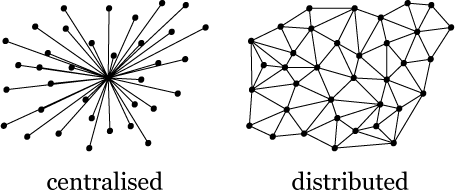
\includegraphics[scale=0.55]{redes}
\caption{Tipos de redes}
\end{figure}

El diseño topológico de una red de estas características es un problema enormemente complejo. En la literatura, la forma de abordar el problema del diseño ha consistido en particionar el problema en dos subproblemas: uno para la red troncal y otro para la red de acceso local. Estos subproblemas se resuelven alternativamente de manera iterativa, solo uno a la vez, mientras los parámetros que pertenecen al otro problema se consideran fijos. Esta aproximación, que podemos encontrar en \cite{bebesita} o \cite{bebesita2}, y a pesar de ser el único válido para redes grandes, tiene el serio inconveniente de no poder garantizar estar siquiera cerca de la solución óptima incluso para un número grande de iteraciones, cada una de las cuales requiere una gran carga computacional.

En este trabajo vamos a abordar el problema del diseño topológico de una red con estructura de dos niveles de jerarquía. Habida cuenta del inconveniente de las aproximaciones clásicas al problema, no particionaremos el problema. Veremos el ataque directo presentado en \cite{paper}, es decir, trataremos de encontrar simultáneamente el diseño óptimo tanto de la red troncal como de la red de acceso local. Con el fin de hacer factible esta aproximación incluso para redes grandes, nos atendremos a redes con la siguiente configuarción:

\begin{itemize}
\item La red troncal es complemante conexa o \textit{full-meshed}.
\item Todas las redes de acceso local adjuntas serán del tipo estrella. 
\end{itemize}

\begin{figure}[h!]
\centering
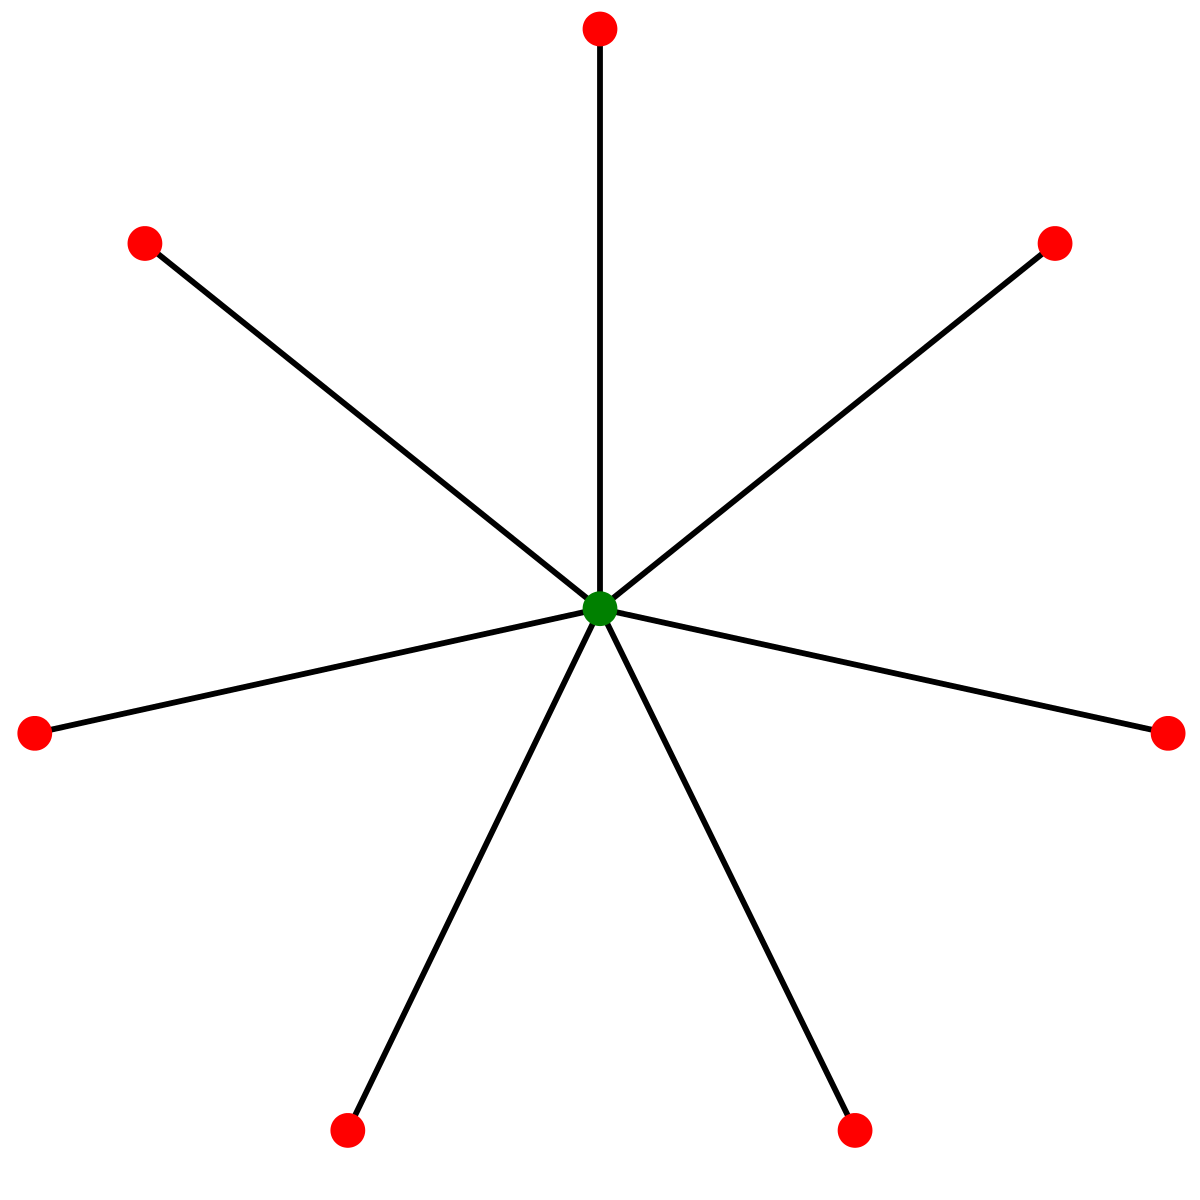
\includegraphics[scale=0.1]{star}
\caption{Ejemplo de grafo de tipo estrella}
\end{figure}
Nos referiremos a los nodos de la red troncal como \textbf{nodos troncales} y a los de la red de acceso local como \textbf{nodos de usuarios}. Nuestro problema puede describirse de la siguiente manera:
\begin{enumerate}[(a)]
\item Se conocen la localización de los nodos de usuarios y los candidatos a ser nodos troncales. 
\item No hay límite al número de nodos de usuario que pueden estar conectados a un nodo troncal.
\item Hay tres tipos de coste asociados: establecer un nodo troncal, interconectar dos nodos troncales establecidos y conectar un nodo de usuario a un nodo troncal.
\end{enumerate}
De esta manera podemos definir dos tipos de variables de decisión: una para determinar el número y localización de nodos troncales y otra para asignar los nodos de usuarios a nodos troncales. Más adelante en la formulación del problema veremos esto con mayor claridad. En pocas palabras, nuestro problema consiste en ubicar con el menor coste posible un subgrafo de la red troncal de manera que todos los nodos de usuario estén conectados.

Quizás alguien podría suponer que la asunción de completitud sobre la red troncal es demasiado restrictiva para poder aplicar el procedimiento en problemas reales. Sin embargo, existe una gran cantidad de redes reales de comunicación cuyas redes troncales son \textit{full-meshed}. De hecho, este tipo de conexiones es casi un prerrequisito para las redes de comunicación en los que la fiabilidad del sistema y/o el tiempo de respuesta son los criterios más importantes para evaluar su rendimiento. Por ejemplo, consideremos una red de señalización por canal común o \textit{common-channel signaling} (CSS), la cual se utiliza para transmitir información de control entre centrales en una red de telecomunicaciones. En la red CSS, los centros especializados corresponden a los nodos troncales. La subred de dichos centros suele ser completamente conexa, dado que no hay ningún criterio a satisfacer más importante que la rapidez y fiabilidad de la transferencia de los mensajes. También podemos encontrar ejemplos en las redes telefónicas en áreas metropolitanas o las redes de transporte con centros de almacenaje. 

Nuestro problema del diseño topológico puede ser visto como una versión generalizada del problema de localización de plantas con capacidad de producción infinita o \textit{uncapcitated facility location problem} (UFLP). La única diferencia con el UFLP es que en nuestra formulación la red de las plantas o instalaciones debe ser completamente conexa, mientras que en el UFLP no todas las plantas tienen que estar necesariamente interconectadas.

\section{Formulación del problema}
En esta sección vamos a ver que el problema del diseño topológico de la red puede ser formulado como un problema de Programación Entera binario, pues nos aparecen términos cuadráticos en la función objetivo. En primer lugar, definamos los elementos involucrados en la formulación.
\begin{itemize}
\item $I=\{1,\dotsc,m\}$ es el conjunto de lugares potenciales para situar nodos troncales.
\item $J=\{1,\dotsc,n\}$ es el conjunto de nodos de usuario.
\item $x_{ij}=1$ si el nodo de usuario $j$ está asignado al nodo troncal $i$ y $0$ en otro caso.
\item $y_i =1$ si establecemos el nodo troncal $i$ y $0$ en otro caso.
\item $c_{ij}$ es el coste no negativo de asignar el nodo de usuario $j$ al nodo troncal $i$.
\item $f_i$ es el coste no negativo de establecer el nodo troncal $i$. 
\item $d_{il}$ es el coste no negativo establecer un enlace entre $i$ y $l$ $(d_{il} = 0$ si $i\geq l$).
\end{itemize}
Entonces, la formulación del problema queda de la siguiente manera.
\begin{align}
\min \,& \sum_{i\in I} \sum_{j\in J} c_{ij}x_{ij} + \sum_{i\in I} f_i y_i + \sum_{i \in I}\sum_{l \in I} d_{ij}y_iy_l\\
s.a.\,& \sum_{i\in I} x_{ij} = 1 \qquad  j \in J\\
& x_{ij}\leq y_i \quad\;\;\qquad i \in I,\; j\in J\\
&x_{ij}\in\{0,1\} \qquad i \in I,\; j\in J\\
&y_i\in\{0,1\} \qquad \;i\in I
\end{align}
Expliquemos los bloques de restricciones. Las restricciones del tipo (2) nos aseguran que cada nodo de usuario está conectado a un único nodo troncal, mientras las que las del tipo (3) garantizan que los nodos de usuarios se asignan a nodos troncales que hayan sido realmente establecidos. A pesar de que cada vez se han reportado más avances en el estudio de programación cuadrática 0-1, la mayoría de ellos están centrados en el caso sin restricciones. Algunos estudios señalables del caso general con restricciones son, por ejemplo, el trabajo de McBride y Yormark \cite{mcbride} donde desarrollan un método  de ramificación y acotación donde las cotas inferiores se obtienen relajando las restricciones 0-1. También Lazimy propone un algoritmo basado en la descomposición de Bender en \cite{lazi}. Sin embargo, el enorme tamaño de los modelos como el nuestro hace que estas técnicas sean computacionalmente prohibitivas. Por esta razón, vamos a utilizar una formulación alternativa equivalente lineal en la que explotamos la estructura particular de nuestro problema.
\newpage
Para linealizar los términos cuadráticos de la función objetivo $y_iy_l$, introducimos las variables 0-1 $z_{il} = y_iy_l$ que satisfacen las restricciones para todo $1\leq i \leq l \leq m$
\begin{align}
&y_i+y_l\leq z_{il}+1\\
&z_{il} \leq y_i\\
&z_{il}\leq y_l\\
&z_{il}\geq 0\\
&z_{il}\in \mathbb{Z}
\end{align}
Sin embargo, notemos que en la formulación particular de nuestro problema las restricciones (7), (8) y (10) son innecesarias, pues, dado que los costes $d_{il}$ son no negativos y estamos minimizando, $z_{il}$ alcanzará necesariamente su valor mínimo en el óptimo. 

Ahora consideremos una extensión del bloque (6) de restricciones. Sea $\{I^k\}_{k\in K}$ el conjunto de los subconjuntos de $I$ tales que $|I^k|\geq 2$. Entonces el siguiente bloque de restricciones generaliza a 6:
\begin{align}
\sum_{i\in I^k} y_i \leq  \sum_{i\in I^k} \sum_{l\in I^k,\,i<l} z_{il} +1 \qquad k\in K
\end{align}
Notemos que las desigualdades del tipo 11 con $|I^k| =2$ son equivalentes a (6) y una desigualdad con $|I^k|\geq 3$ es redundante. Sin embargo, si reemplazamos (11) por (6), la relajación lineal del problema será al menos tan ajustado como la formulación de (6). Es más, se tiene el siguiente teorema.
\begin{theorem}Todas las desigualdades del tipo (11) definen facetas del politopo entero descrito por las desigualdades (6)-(10). 
\end{theorem}
Por tanto, vamos a enfrentarnos al problema de programación entero mixto 0-1, al que denominamos (P), dado por
\begin{align*}
\min \,& \sum_{i\in I} \sum_{j\in J} c_{ij}x_{ij} + \sum_{i\in I} f_i y_i + \sum_{i \in I}\sum_{l \in I} d_{ij}z_{il}\\
s.a.\,& \text{(2), (3), (4), (5), (9) y (11)}
\end{align*}
\section{Método de solución}
Como en otro caso de programación entera mixta 0-1, vamos a utilizar técnicas de ramificación y acotación. La eficiencia computacional de este tipo de algoritmos va a depender en gran medida de nuestra capacidad para generar buenas cotas inferiores. En nuestro caso, veremos el desarrollo de un procedimiento eficiente para obtener dichas cotas para el problema utilizando las siguientes características propias de su estructura.
\subsection{Estructura del problema}
El número exponencial de desigualdades del tipo (11) hace imposible incorporar todas ellas a la relajación lineal inicial. La aproximación pragmática consiste en generar desigualdades solo cuando se necesitan, de la misma forma se utiliza en los algoritmos planos de corte. Para este propósito, necesitamos un procedimiento para generar desigualdades del tipo (11) y resolver sucesivamente el problema de programación lineal resultante de añadir una nueva desigualdad.

Es más, nuestro problema sin las restricciones (11) es precisamente un UFLP, el cual tiene una estructura dual interesante. Explotando esta estructura especial, Bilde y Karup \cite{bilde} han desarrollado método dual el cual está ampliamente aceptado como el más potente. Denotemos $K(i) = \{k \in K \mid i \in I^k\}$ para todo $i\in I$. Sea además $K(i,l) = K(i)\cap K(l)$ para todo $i,l \in I$ tal que $i<l$. El dual de nuestro problema relajando las condiciones (4) y (5), convirtiéndolo en un problema de programación lineal, está dado por:
\begin{align*}
\max \,& \sum_{j\in J} v_j - \sum_{k\in K} \gamma_k \\
s.a.\,& v_j - w_{ij} \leq c_{ij} \qquad  i\in I,\;j \in J\\
& \sum_{j\in J} w_{ij} - \sum_{k\in K(i)} \gamma_k \leq f_i \;\qquad i \in I,\; j\in J\\
&\sum_{k\in K(i,l)} \gamma_k \leq d_{il} \qquad i \in I,\; l\in I,\; i<l\\
&w_{ij},\gamma_k \geq 0 \qquad \;i\in I,\; j\in J,\; k\in K
\end{align*}
donde $v_j$, $w_{ij}$ y $\gamma_k$ son las variables duales asociadas a las restricciones (2), (3) y (11) respectivamente. Para cada elección factible de $v_j$ y $\gamma_k$, cada variable $w_{ij}$ puede tomarse como su menor valor posible dado por $w_{ij} = \max\{0,v_j-c_{ij}\}$. Entonces el problema anterior se puede reemplazar por esta forma condensada, a la que denominamos (D).
 \begin{align*}
\max \,& \sum_{j\in J} v_j - \sum_{k\in K} \gamma_k \\
s.a.\,& s_i:= f_i -\sum_{j \in J} \max\{0,v_i-c_{ij}\} + \sum_{k \in K(i)} \gamma_k \geq 0 \;\quad  i \in I \\
& s_{il}:= d_{il} - \sum_{k\in K(i,l)} \gamma_k \geq 0 \qquad i \in I,\; l\in I,\; i<l\\
&\gamma_k \geq 0 \qquad  k\in K
\end{align*}
Dado un conjunto de valores de $\gamma$ para el problema (D), el problema resultante se denomina forma condensada dual del UFLP. Podemos construir los valores $v_j$ directamente usando heurísticas desarrolladas también en \cite{bilde}. Este proceso cicla repetidamente los $j\in J$ intentando incrementar $v_j$ desde un valor de $c_{ij}$ al siguiente mayor valor posible. Si para algún valor $j$ el incremento viola la factibilidad, $v_j$ se incrementa solo hasta el mínimo que permitan las restricciones de $s_i$. Cuando todos los $v_j$ son tales que no pueden ser incrementados, entonces hemos terminado.
\newpage
\subsection{Procedimiento de ramificación y acotación}
Como ya hemos comentado, resolveremos la relajación lineal de (P) iterativamente utilizando el método la heurística anterior. Denotemos por $K^t$ el subconjunto de $K$ de índices de $I^k$'s correspondientes a las desigualdades del tipo (11) que han sido generadas antes de la iteración $t$. Denotemos por $(P^t)$ el problema correspondiente a (P) reemplazando $K$ por $K^t$ y por $(D^t)$ el dual de $(P^t)$. En cada iteración $t$, obtenemos una solución factible $(D^t)$ y también una solución entera factible para (P). En el caso de que nuestra solución no sea óptima, generamos una desigualdad del tipo (11) usando una solución dual de $(D^t)$. Para seleccionar dicha desigualdad nuestro criterio debe ser tal que al añadirla a la relajación lineal de $(P^t)$ provoque un aumento de la correspondiente variable dual $\gamma_k$. 

El incremento de $\gamma_k$ crea una holgura $s_i$ para $i\in I^k$ que puede resultar en un incremento de alguna $v_j$. Si más de un $v_{j}$ puede ser incrementado para cada incremento de un $\gamma_{k}$, el valor objetivo dual también será incrementado. Notemos que el incremento de $s_{i}$ que, en la etapa actual, tiene valor igual a cero es el mejor candidato para incrementar $v_{j}$. Es más, el incremento de $\gamma_{k}$ está restringido por la holgura de $s_{il}$. Por tanto, elegiremos como candidato un conjunto $I^{k}$ que satisfaga las condiciones siguientes:
\begin{enumerate}[1.]
    \item $I^{k}\subseteq I^{*}=\{i\in I:s_{i}=0\}$ con $|I^{k}|\geq 2$.
    \item $s_{il}>0$ para todo $i, \ l\in I^{k}$ tal que $i<l$.
    \item $I^{k}$ no está contenido en ningún otro conjunto que satisfaga 1 y 2.
\end{enumerate}

Sea $G(V,E)$ el grafo asociado a (D) que tiene un nodo por cada $i\in I$ y una arista por cada par $i,l \in I^{*}$ con $s_{il}$ positivo. Entonces seleccionar un $I^{k}$ que satisfaga las tres condiciones anteriores es equivalente a seleccionar un \textbf{clique} en $G$. En primer lugar, establecemos $I^{k}=\{i\}$ eligiendo un $i\in I^{*}$ inicial, que llamaremos \textbf{nodo semilla}, y lo aumentaremos sucesivamente con $l\in I^{*}/I^{k}$ tal que $s_{l}=0$ y $s_{il}(o\ s_{li})>0$ para todo $i\in I^{k}$. Gracias a las propiedades de un clique, podemos construir uno sin repetición, para ello basta elegir un nodo semilla entre los nodos troncales que no estén contenidos in ningún clique generado anteriormente.\\

En cada iteración, para unos $s_{i}$ y $s_{il}$ dados, elegimos arbitrariamente un subconjunto de $I^{*}$ que forme un clique tal como indicamos en el párrafo anterior. Ahora determinamos el máximo incremento posible de $\gamma_{k}$, cada uno de los cuales provocando que uno o más $v_{j}$ incrementen conjuntamente con el incremento de $s_{i}$ para $I\in i^{k}$, al mismo tiempo que mantengan factibles las condiciones (13). Para lograrlo, incrementamos primero cada $s_{i}$ para $i\in I^{k}$ usando $\delta=min\{s_{il}:i,l \in i^{k},\ i<l\},$ e incrementado entonces los $v_{j}$ mediante la heurística ascendente dual. Finalmente, determinamos el incremento de $\gamma_{k}$ como la \textbf{máxima holgura absorbida}, es decir, $\Delta\gamma_{k}=\delta-min_{i\in I^{k}}s_{i}$.\\

Usando este procedimiento, por cada unidad incrmentada de $\gamma_{k}$, se incrementa una unidad en al menos uno de los $v_{j}$, lo que hace que el valor objetivo dual no disminuya nunca. Con cada iteración se obtiene además una solución primal entera y factible gracias a la heurística primal ¿add-type?. Primeros incluimos un nodo troncal $i\in I^{*}$ que tenga el mayor número de aristas con $s_{il}=0$ en $G$ dentro del conjunto de nodos troncales abiertos. Ahora se añaden otros nodos troncales en $I^{*}$ con la intención de mejorar el coste total.\\

Para acelerar todo el proceso, limitamos la elección de los nodos semilla. Cuando implementemos una desigualdad correspondiente a un $I^{k}$, si el $\gamma_{k}$ asociado no incrementa una cantidad $\delta$ o su implimentación no mejora el valor objetivo dual, eliminamos en los nodos troncales contenidos en $I^{k}$ el conjunto de nodos semilla candidatos para las siguientes iteraciones. Esto evitará la elección de un clique cuyos nodos estén completamente contenidos en $I^{k}$, puesto que el incremento adicional de $s_{i}$ para un subconjunto de nodos troncales estrictamente contenidos en $I^{k}$ tiene pocas posibilidades de mejorar el valor objetivo dual en las iteraciones siguientes. El procedimiento se describe a continuación:

$Paso \ 0$. Inicializar con cualquier solución factible $\{v_{j}\}$ de $(D^{0})$ y fijar $s_{i}$ y $s_{il}$ como en (12) y (13). Establecemos $\text{CAND}=I^{*}$.\\

$Paso\ 1$. Elegir un nodo semilla $i\in$ CAND. Si CAND es un conjunto vacío, entonces STOP.\\

$Paso\ 2$. Construir un $I^{k}$ usando el nodo semilla elegido. Si el conjunto anterior no existe, entonces $\text{CAND}=\text{CAND}\setminus\{i\}$ e ir al Paso 1. En caso contrario:
\begin{enumerate}[a.]
    \item para $i\in I^{k}$, incrementar $s_{i}$ una catidad $\delta=min\{s_{il}:i,l\in I^{k},i<l\},$
    \item aplicar la heurística ascendente dual,
    \item calcular el incremento de $\gamma_{k}$ y actualizar $s_{il}$:
        \begin{center}
        $\Delta\gamma_{k}=\delta-min_{i\in I^{k}}s_{i},\newline
        s_{il}\leftarrow s_{il}-\Delta\gamma_{k}$ para $i,l\in I^{k},\ i<l$,
        \end{center}
    \item si $\Delta\gamma_{k}\neq\delta$, ajustar $s_{i}$ para $i\in I^{k}$:
        \begin{center}
        $s_{i}\leftarrow s_{i}-min_{i\in I^{k}} s_{i}$.
        \end{center}
\end{enumerate}


$Paso\ 3$.Construir una solución primal entera y factible y actualizar la solución asociada si es posible.\\

$Paso\ 4$. Si $\Delta\gamma_{k}\neq\delta$ o el valor objetivo dual no ha mejorado, entonces establecemos $\text{CAND}=\text{CAND}\setminus\{I^{k}\}$, y volver al Paso 1.\\


Estos procedimientos, aplicados al primal y al dual, permiten obtener cotas superiores e inferiores de (P). Si existe un espacio entre ellos, pasamos a un proceso de ramificación y acotación. Es ese caso, adoptaremos un esquema de vuelta atrás donde el último nodo que haya entrado será el primero en salir. Para la ramificación aplicamos el mismo criterio que usamos para seleccionar el primer nodo troncal abierto en la heurística primal. En \cite{Erlen} se propone una manera de actualizar eficientemente la solución factible dual en cada iteración para el problema obtenido tras la ramificación. Usaremos esta estrategia (propuesta por Erlenkotter) con la salvedad de que, en nuestro caso, resetearemos todos los $\gamma_{k}$ a cero antes de ramificar. Además, al resolver los problemas parciales (asociados con cada ramificación) donde fijemos algún nodo troncal abierto, aplicamos una regla de prioridad para establecer una desigualdad (11). Dicha regla consiste en elegir en primer lugar un clique tal que contenga un nodo troncal abierto fijo.\\
\newpage
\begin{thebibliography}{9}
\bibitem{bebesita}
Boorstyn, R.R., and Frank, H., "Large-scale network
topological optimization", IEEE Transactions on Communications
25 (1977) 29-47

\bibitem{bebesita2}
Gavish, B., "Topological design of centralized computer
networks - formulation and algorithms", Networks 12
(1982) 355-377. 
\bibitem{mcbride}
McBride, R.D., and Yormark, J.S., "An implicit enumeration algorithm for quadratic integer programming", Management Science 26 (1980) 282-296.

\bibitem{lazi}
Lazimy, R., "Improved algorithm for mixed-integer quadratic programs and a computational study", Mathematical Programming 32 (1985) 100-113.

\bibitem{bilde}
Bilde, O. and Krarup, J., "Sharp lower bounds and
efficient algorithms for the simple plant location problem",
Annals of Discrete Mathematics 1 (1977) 314-325.

\bibitem{paper}
Chung, Sung-hark; Myung, Young-soo; Tcha, Dong-wan. (1992). Optimal design of a distributed network with a two-level hierarchical structure. European Journal of Operational Research. 62. 105-115. 10.1016/0377-2217(92)90181-8. 

\bibitem{Erlen}
Erlenkotter, D., "A dual-based procedure for uncapacitated
facility location", Operations Research 26 (1978)
992-1009.
\end{thebibliography} 
\end{document}